% Online实际参数放置与归胞后的侧视；只裁切原JPEG，不修改像素。
\begin{figure}[H]
\centering
% 3024×1758；(980,620,2045,1480)，1065×860；107mm约253ppi。
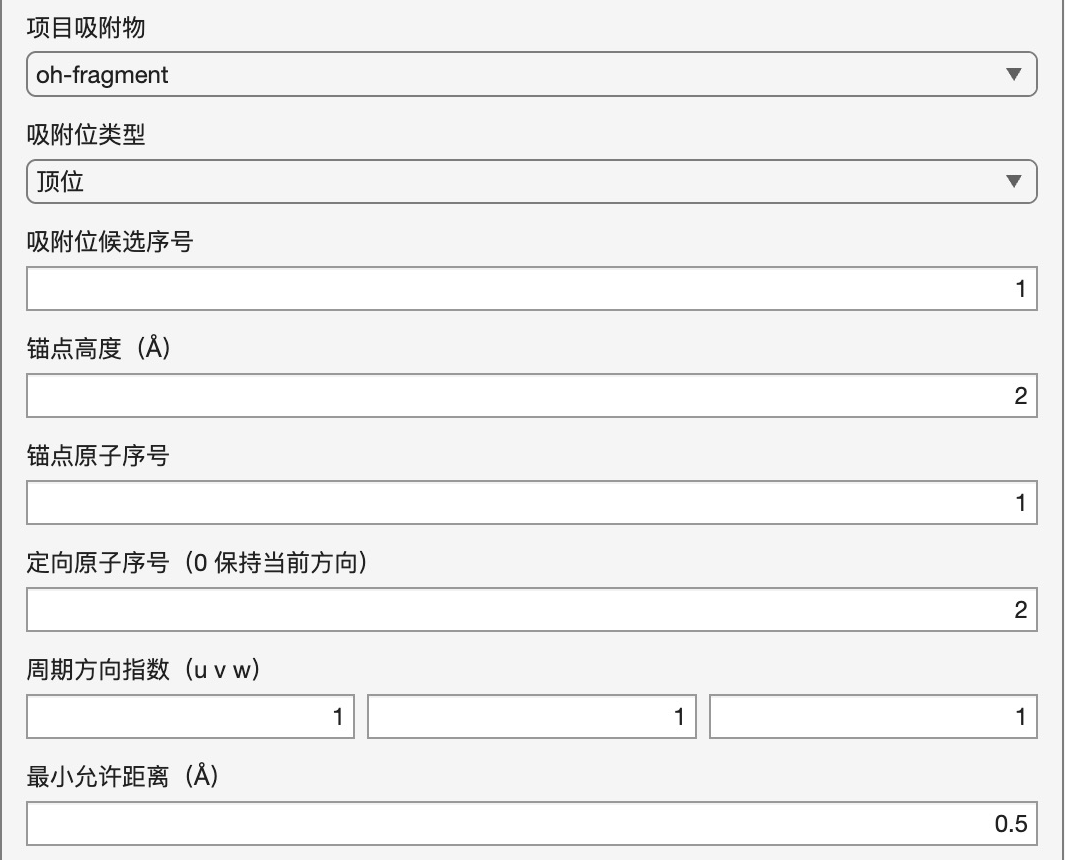
\includegraphics[width=107mm]{publication-assets/crop-c02e14aa8762e8947bbe.png}
\caption{Online中向外放置O--H的实际参数。选择项目中的\file{oh-fragment}，顶位候选1，锚点高度$2\,\text{\AA}$，锚定原子1、定向原子2，周期方向指数依次为1、1、1，最小允许距离$0.5\,\text{\AA}$。本例已先将宿主的$c$调整为表面法向。}
\label{fig:pt111-oh-parameters}
\end{figure}

\begin{figure}[H]
\centering
\begin{minipage}[t]{80mm}
\vspace{0pt}
% 完整晶胞(1000,360,2020,1685)，1020×1325；80mm约324ppi。
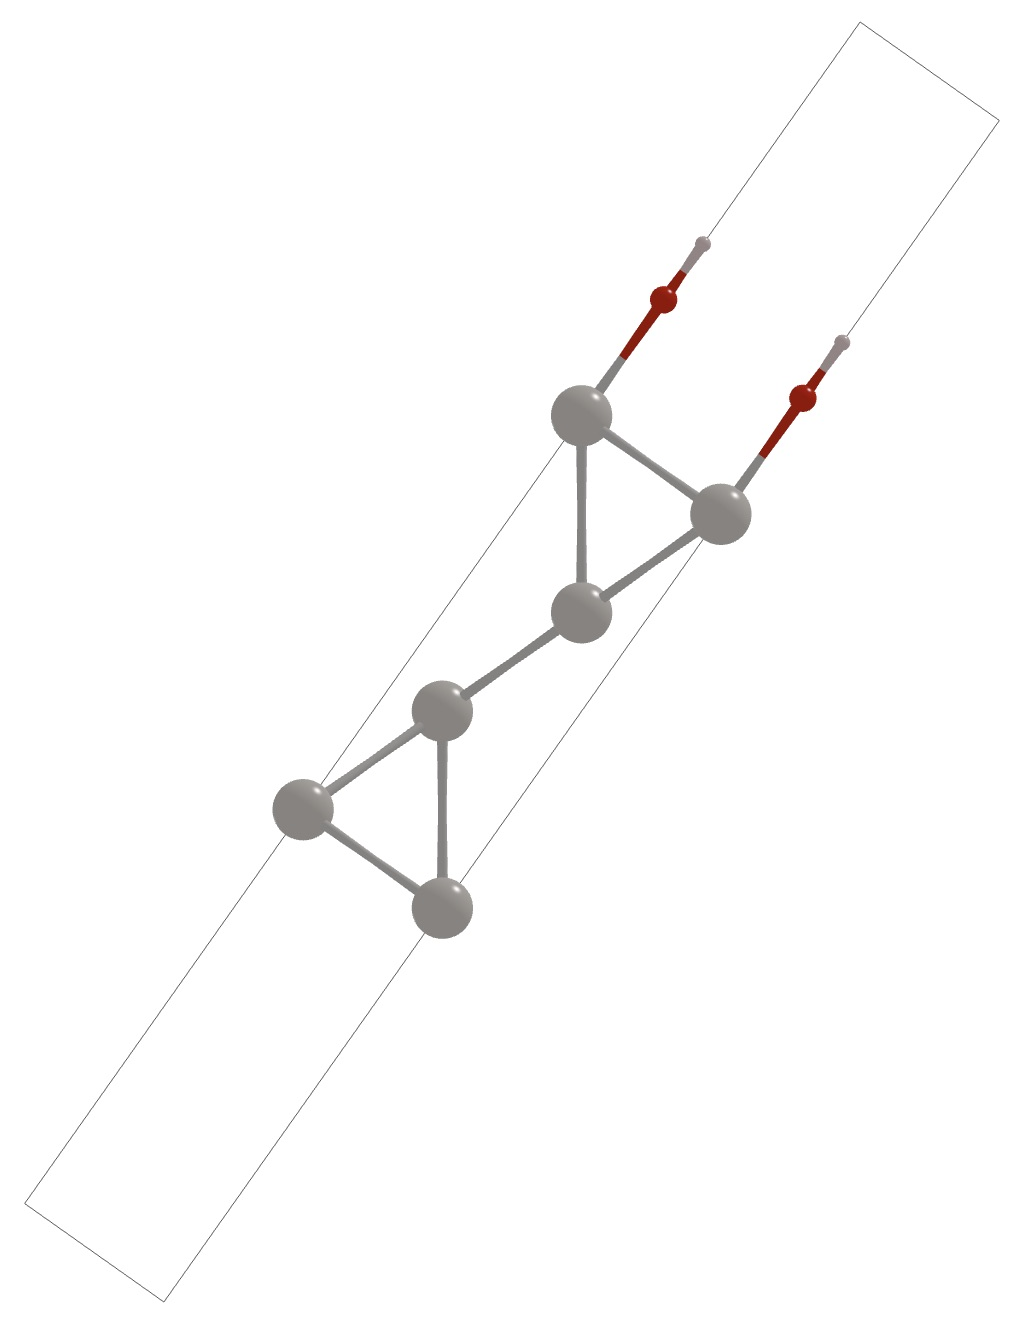
\includegraphics[width=\linewidth]{publication-assets/crop-c201c0495d5d847c2fd3.png}
\end{minipage}\hfill
\begin{minipage}[t]{40mm}
\vspace{0pt}
% 独立摘要(40,330,445,560)，405×230；40mm约257ppi。
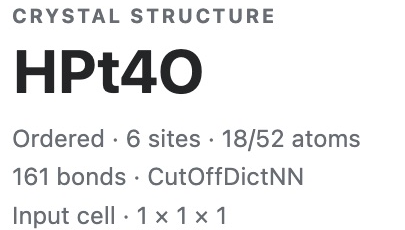
\includegraphics[width=\linewidth]{publication-assets/crop-5caa5064e4762ffc4974.png}
\end{minipage}
\caption{应用吸附放置并以$1\times1\times1$单位超胞归胞后的Online侧视。摘要确认$\mathrm{Pt_4OH}$、6个独立位点；画面中的两个O--H是同一片段的周期显示映像。显示原子数为18/52，不能据此把模型组分读作两个O--H。图中结构仅为已放置的初始几何。}
\label{fig:pt111-oh-side}
\end{figure}
